\subsection{Test vehicle description}
\label{sec:test-vehicle-desc}

% A testchip has been made to put measurement structures on silicon
Integrated circuits are very dense and fragile devices, enclosed in plastic or ceramic packages.
It is nearly impossible to measure electrical properties without physical access.
For instance, it could be useful to measure potential inside a given net inside the circuit.
With integrated circuits, this is not doable and most of the time the external connections are the only points of access.
Even with physical internal access, placing micro-probes to contact metal connections can disturb sensitive parts of the device.
To overcome these issues, new approaches are required.
In this research, custom measurement structures have been implemented directly on-chip.
They perform analog measurements at the silicon level.
External interaction with the structure to configure them and read the measurement data is done with digital input/output.
The global architecture of the testchip is provided in Fig. \ref{architecture_testchip}.
It contains two instances of the regulation function studied earlier in \ref{sec:study-real-product}.
The first instance is exposed to \gls{ESD} stresses during tests and is monitored for failures.
The second instance powers the monitoring functions and custom measurement structures.
The rest of the chip is composed of the custom structures or communication buses.

\begin{figure}[h]
  \centering
  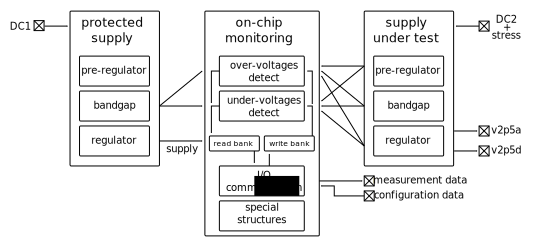
\includegraphics{src/3/figures/architecture_testchip.pdf}
  \caption{Global architecture of the test vehicle}
  \label{architecture_testchip}
\end{figure}

% Isolation between supplies
The protected primary regulator on the left (Fig. \ref{architecture_testchip}) is responsible for powering the monitoring blocks.
It must not be disturbed by the discharges injected on the supply under test on the right.
It has its own external supply pin DC\textsubscript{1}, powered externally by a different DC supply than the regulation function under test.
Large external filtering has been used for this instance.
Except for the ground connection, both regulators do not share connections.

% What is in the monitoring system
The on-chip monitoring system is composed of several overvoltage and undervoltage detectors.
They monitor multiple net voltages inside the supply under test.
There are in total 35 detectors in the testchip.
The purpose of each detector is given in appendix \ref{apx:testchip-register-maps}.

% What is in the communication system
The communication systems provides a connection between the internal detectors and the external world.
Configuration data can be provided from an external microcontroller and measurement data is output by the communication block.

% How those monitoring functions have been designed
The implementation of each monitoring function is detailed hereafter.

\subsection{Voltage monitoring}

% What are the OV/UV detectors made of
Overvoltage and undervoltage detectors are implemented as latched comparators.
A flag is raised if a monitored net crosses a threshold, and stored using a latch, until it can be read.
The architecture of a single detector is given Fig. \ref{fig:architecture-ov}.
The same architecture is used for the overvoltage and the undervoltage.
Monitored and reference inputs are just inversed on the undervoltage detector.

\begin{figure}[!h]
  \centering
  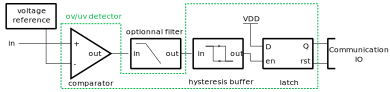
\includegraphics[width=0.9\textwidth]{src/3/figures/architecture_OV.pdf}
  \caption{Architecture of the overvoltage detector}
  \label{fig:architecture-ov}
\end{figure}

% Detail architecture
The first block in this detector is the comparator.
It is designed with a two-stage operational amplifier with an output buffer (see Fig. \ref{fig:comparator-design}).
This topology is well suited for high-gain, open-loop comparators.
This comparator provides a very high input impedance, to ensure the monitored net is not disturbed.
A high-gain is useful for limiting the comparator's offset.
The performance of the comparator is given in table \ref{tab:comparator-performance}.
The critical factors are the high to low delay, to detect very fast transients, and the offset, to ensure detection accuracy is good.

\begin{figure}[!h]
  \centering
  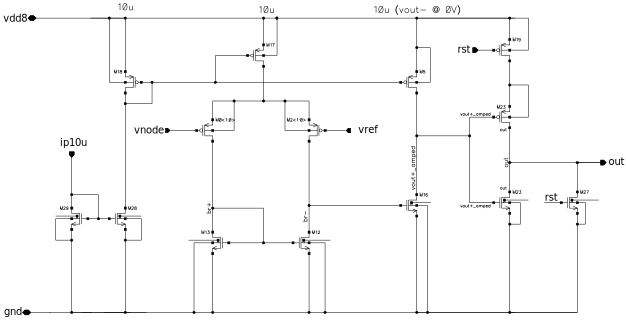
\includegraphics[width=0.9\textwidth]{src/3/figures/comparator_design_clean.pdf}
  \caption{Comparator design}
  \label{fig:comparator-design}
\end{figure}

%TODO: Detail nets of the schematic

\begin{table}[!h]
\centering
\begin{tabular}{@{}lllll@{}}
\toprule
property           & specification & value (typical) \\
\midrule
offset             & +/- 10mV      & 2.65 mV \\
V(IH)              & +/- 10mV      & 1.15 mV \\
V(IL)              & +/- 10 mV     & 4.16 mV \\
delay low2high     & 50 ns         & 41 ns   \\
delay high2low     & 50 ns         & 12.8 ns \\
consumption (dc)   & 60 uA         & 33 uA \\
consumption (peak) & 350 uA        & 264 uA \\
\bottomrule
\end{tabular}
\caption{Comparator performance (typical)}
\label{tab:comparator-performance}
\end{table}


% What is the purpose of filter
On the output of the comparator, an optional RC filter can be connected.
This filter can deglitch very short overvoltages, to only let large overvoltages pass through the detector.
The stratety behind this filter is to use multiple detectors monitoring the same net, each one with a different filter.
In function of which detectors triggered, an estimation of the overvoltage length can be made.

% Hysteresis buffer
After the filter, an hysteresis buffer increases the deglitching action of the filter.
If the comparator's output remains high for a short period of time, the output of the filter will rise slowly.
If a standard buffer was used in place of the hysteresis buffer, it would latch at about half the supply voltage.
With the hysteresis, the buffer switches at a voltage much closer from the supply.
With the same RC filter, this results in a much longer deglitching time.
This was done because RC-filters require large resistors and large capacitors for integration on silicon, and occupy a considerable area on the chip.
By increasing the deglitching time, smaller RC-filters could be used.

% Latch
Finally, the latch stores the overvoltage flag.
By default, the latch is reset at $t=0$.
Its copy input $D$ is connected to the supply.
If the hysteresis buffer triggers high, the enable pin triggers a copy in the latch.
The output $Q$ copies the value from the $D$, storing a logical high in the latch.

% Origin of reference voltages
The reference voltages for these comparators come from either fixed-values set by the protected supply, or \gls{dac} that can be reconfigured through the communication system.

\subsection{Communication system}
\label{sec:comm-system-testchip}

% Why a comm IO
The testchip requires many pins for basic functionnality, such as supplies, grounds, substrate connections, regulation functions.
The manufacturing process for test vehicles enforces an LQFP-48 package.
With the given requirements, this does not leave much pins available for directly outputting monitoring data.
A custom communication bus was designed to reduce the pin count.
Initially, the JTAG (TODO: ref or gloss ?) protocol was envisionned for this application.
However, JTAG requires to use a digital state-machine for operation.
This requires digital-synthesis (TODO: glos), which was not available with our given resource constraints.
Instead, a simplified serie to parallel protocol has been designed from scratch.

% What does the comm IO
Two read-only and two write-only communication buses are implemented on the testchip.
Read-only buses are connected to overvoltage and undervoltage detectors, for reading them.
Write-only buses are connected to configuration registers for some monitoring functions.
For instance, the variable voltage references for the detectors can be set using this bus.

% Why two buses each
A pair of read/write bus serves to validate some monitoring blocks.
The second pair is connected to the actual monitoring function.

% Overall architecture
Each bus is constituted of individual identical cells.
The main principle is to propagate an enable signal.
Each time a cell receives the enable signal, it will perform its duty, wait for a delay, then pass the enable to the next cell.
%TODO: Talk about scalability
%TODO: Speak about JTAG
%TODO: Explain why custom solution and not digital-synthesis
%TODO: Talk about comm not being used during the ESD, but afterward


\subsubsection{Read cell}

% Explain behavior
The read cell is constituted of a tri-state buffer and a D-latch (see Fig. \ref{fig:read-cell-design}).
The output of the tri-state buffer is set in high-impedance when the \textit{x} input is low.
This action releases the communication bus for other read cells and is the default state.

% Chaining
Multiple cells can be connected serially in a chain-fashion.
Increasing the total register size is simply done by adding more cells to the chain.
This is convenient for testchip developments that have limited design resources.

\begin{figure}[!h]
  \centering
  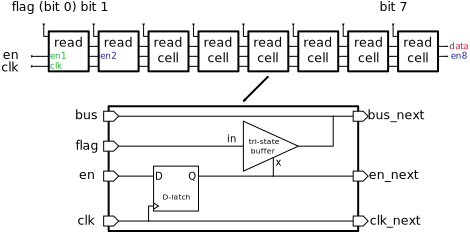
\includegraphics[width=0.5\textwidth]{src/3/figures/architecture_read_cell.pdf}
  \caption{Read-only cell design}
  \label{fig:read-cell-design}
\end{figure}

% Describe the chronogram
Fig. \ref{fig:read-cell-curve} shows the simulated behavior of a chain of 8 reading cells.
Signals in green (\textit{en\_in} and \textit{clk}) must be provided externally, by a microcontroller for instance.
Signals in blue are internal control signals, to help the cells determine if they have the right to write on the bus.
The signal in red (\textit{ser\_out}) is the data output, read by an external microcontroller.

% Explain time-response
The reading sequence is initiated by setting \textit{en\_in} high.
When \textit{en\_in} is set high, the output of the first latch (\textit{en\_out\_1}) switches high at the next clock cycle.
This means the first cell has the permission to write on the bus.
During one clock cycle, the \textit{flag} is written on \textit{ser\_out}.
At the next clock cycle, the enable signal is propagated to the next cell.
The first cell no longer has the permission to write to the bus.
The second cell writes to the bus, during a single clock cycle.
The process is naturally repeated by the system, until the enable has been propagated to the last cell (\textit{en\_out\_8}) and all serial data was written.

\begin{figure}[!h]
  \centering
  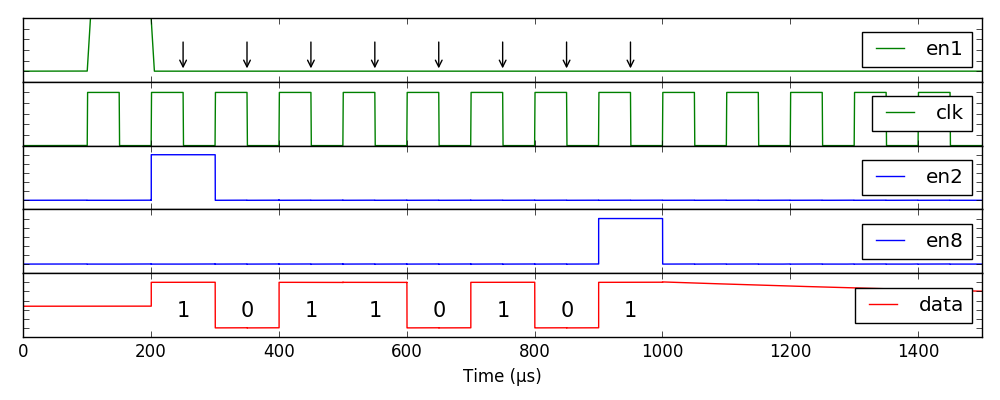
\includegraphics[width=0.95\textwidth]{src/3/figures/curve_read_cell.png}
  \caption{Chronogram for the read cell}
  \label{fig:read-cell-curve}
\end{figure}

\subsubsection{Write cell}

% Explain behavior
The write cell is a bit more complex but operates on the same principle (Fig. \ref{fig:write-cell-design}).
Data is placed serially by the user on the \textit{bus} line, syncronously with the clock.
The enable signal is propagated from cell to cell, so that each cell knows when to sample the bus line and store the value.
Basically, this cell sets on the \textit{output} the value on the bus when its enable is high (Fig. \ref{fig:write-cell-curve}).

\begin{figure}[!h]
  \centering
  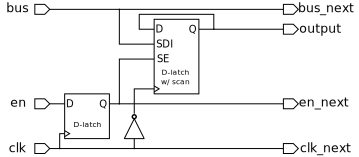
\includegraphics[width=0.5\textwidth]{src/3/figures/architecture_write_cell.pdf}
  \caption{Write-only cell design}
  \label{fig:write-cell-design}
\end{figure}

% Detail devices
The truth table of this latch is given in table \ref{tab:d-latch-scan-truth}.
D1 is a synchronous D-latch.
The output Q copies the input D on rising clock edges.
D2 is a synchronous D-latch with scan.
The output Q copies the data input D on rising clock edges, storing a value.
When the scan enable \textit{se} input is HIGH, the data input D copies the value of the scan data input (\textit{SDI}), effectively changing the stored value.

\begin{table}[!h]
\centering
\begin{tabular}{@{}lllll@{}}
\toprule
D  &  SDI  &  SE  &  CLK  &  Q \\ \midrule
0  &  -    &  0   &  \nearrow    &  0 \\
1  &  -    &  0   &  \nearrow    &  1 \\
-  &  0    &  1   &  \nearrow    &  0 \\
-  &  1    &  1   &  \nearrow    &  1 \\
-  &  -    &  -   &  \searrow    &  Q \\
\bottomrule
\end{tabular}
\caption{D-latch with scan truth-table}
\label{tab:d-latch-scan-truth}
\end{table}

\begin{figure}[!h]
  \centering
  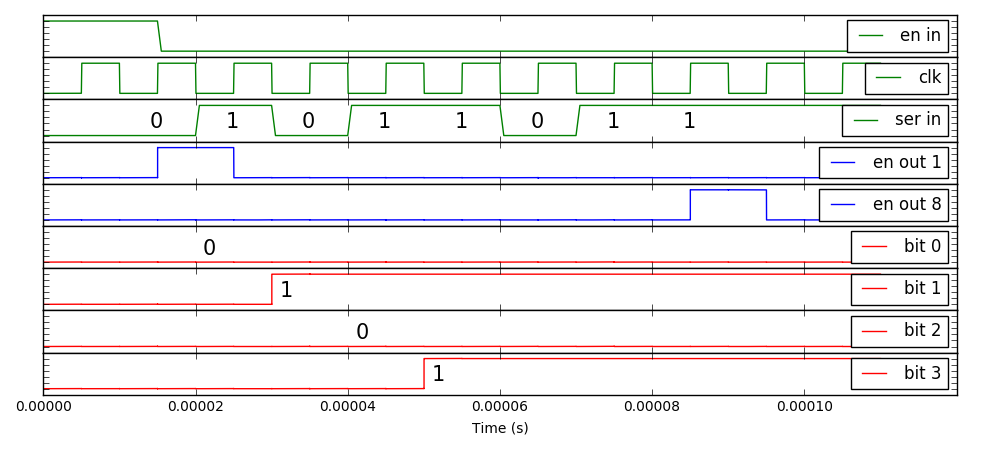
\includegraphics[width=0.95\textwidth]{src/3/figures/curve_write_cell.png}
  \caption{Chronogram for the write cell}
  \label{fig:write-cell-curve}
\end{figure}

% Describe the chronogram
Fig. \ref{fig:write-cell-curve} shows the simulated behavior of a chain of 8 writing cells.
Signals in green (\textit{en\_in} and \textit{clk}) must be provided externally.
Signals in blue are internal control signals, to help the cells determine if to who belongs the data on the bus.
The signals in red (\textit{ser\_out}) are the data output, set on each individual output bit.
Ultimately, the reading-cell performs a serial to parallel conversion.
The serial data is set on \textit{ser\_in}, and the parallel outputs are \textit{bit0},\textit{bit1}, etc.

\subsubsection{Register map}

The complete register maps of readable and writable data is given in appendix \ref{apx:testchip-register-maps}.
%TODO: Detail more ? amount of readable bits, writeable bits, registers

\subsection{On-chip near-field current sensors}
%TODO: Add reference to article ESREF 2012

% Measuring currents is important too
All monitoring structures presented so far watch for voltages.
There is no measurement or monitoring function for currents.
To this goal, current sensors were integrated on silicon, on a few critical nets.

% What is a current sensors
In this testchip, the current sensor is a near-field current loop.
The sensor is placed close to a metal track in which current must be measured.
By coupling, the sensor generates a voltage proportional to the derivative of the current in the track.

Figure. \ref{fig:near-field-current-sensor} and \ref{fig:near-field-current-sensor-layout} gives respectively a visual representation of the sensor and the final layout.
This kind of integrated loop was originally designed and studied in \cite{AlainSallesInductors}.

\begin{figure}[!h]
  \centering
  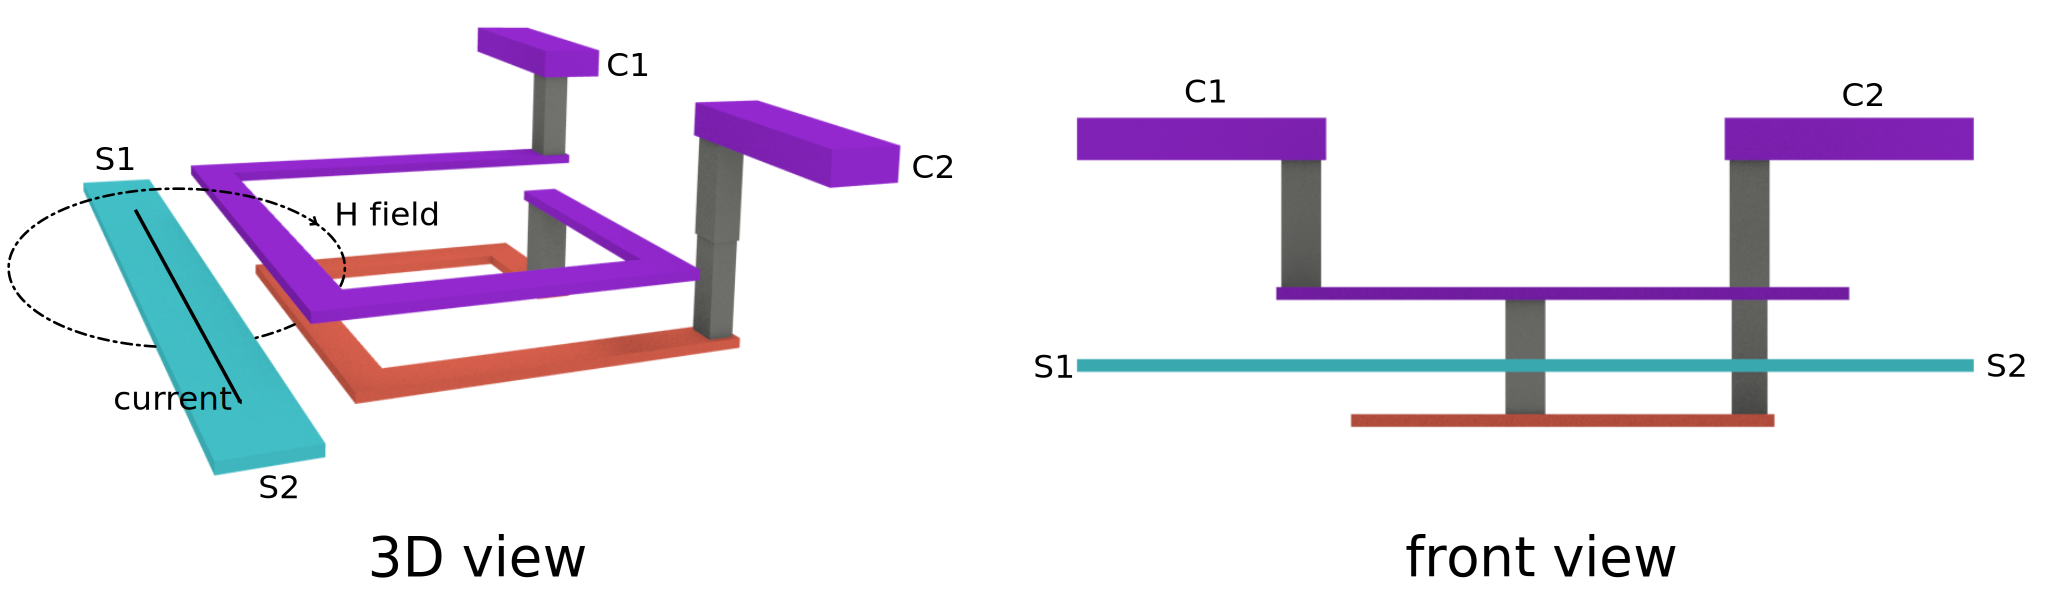
\includegraphics[width=0.98\textwidth]{src/3/figures/near-field-current-sensor.pdf}
  \caption{Near-field current sensor design}
  \label{fig:near-field-current-sensor}
\end{figure}

\begin{figure}[!h]
  \centering
  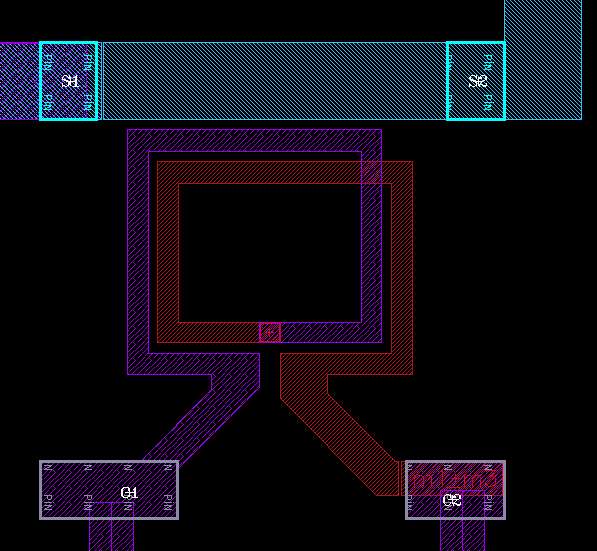
\includegraphics[width=0.5\textwidth]{src/3/figures/sensor_layout.png}
  \caption{Near-field current sensor layout}
  \label{fig:near-field-current-sensor-layout}
\end{figure}

% How is it designed and how is it used
On silicon, three levels of metal are used to build the sensor.
The first level (in red) and the third level (in purple) form a metal loop.
Metallic vias connect both levels to close the loop vertically.
Finally, the sensed current is at the second level (pale blue), and circulates between nets \textit{S1} and \textit{S2}.
An oscilloscope with 50\textOmega\ input impedance performs a differential voltage measurement between pins \textit{C1} and \textit{C2}.
An example waveform obtained by injecting a rectangular pulse is given in Fig. \ref{fig:nfs-wvf}.
The obtained waveform requires specific post-processing to reconstitute the original current waveform.
The post-processing is detailed later in section \ref{sec:on-chip-near-field-process}.

\begin{figure}[!h]
  \centering
  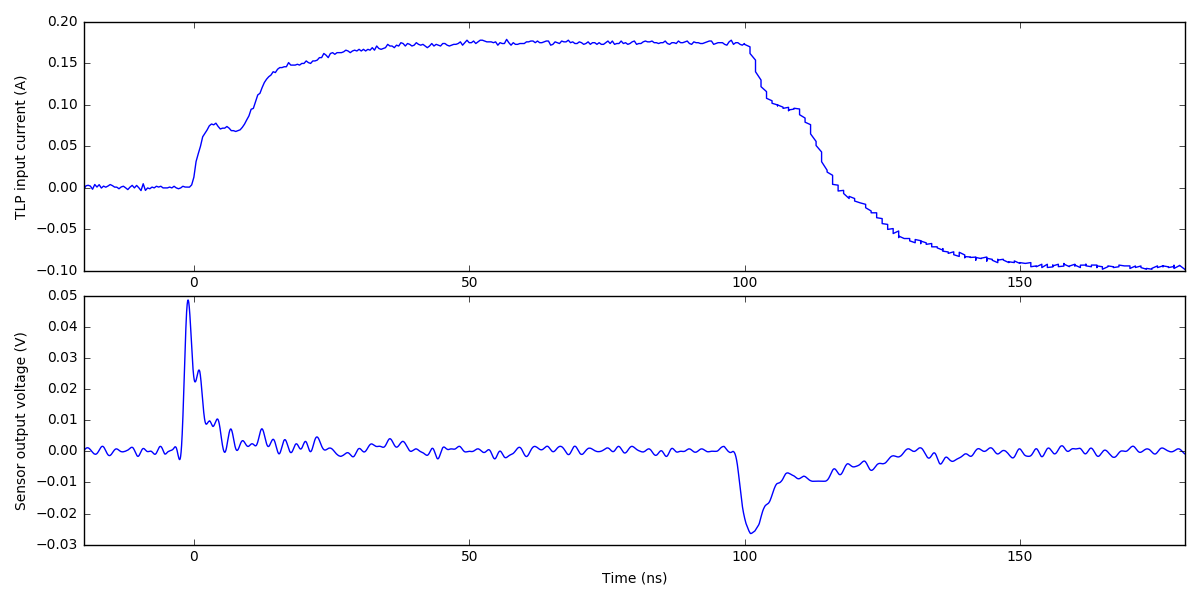
\includegraphics[width=0.9\textwidth]{src/3/figures/measured_waveform.png}
  \caption{Measured waveform with the on-chip near-field sensor}
  \label{fig:nfs-wvf}
\end{figure}

\subsection{Topcell}
% intro
Except for the two supply blocks, all the functionnalities described previously were designed, simulated and layouted.
All layouts were assembled together to form the topcell (Fig. \ref{fig:top-cell-layout}).
The complete pinout is given in appendix \ref{apx:testchip-pinout}.

\begin{figure}[!h]
  \centering
  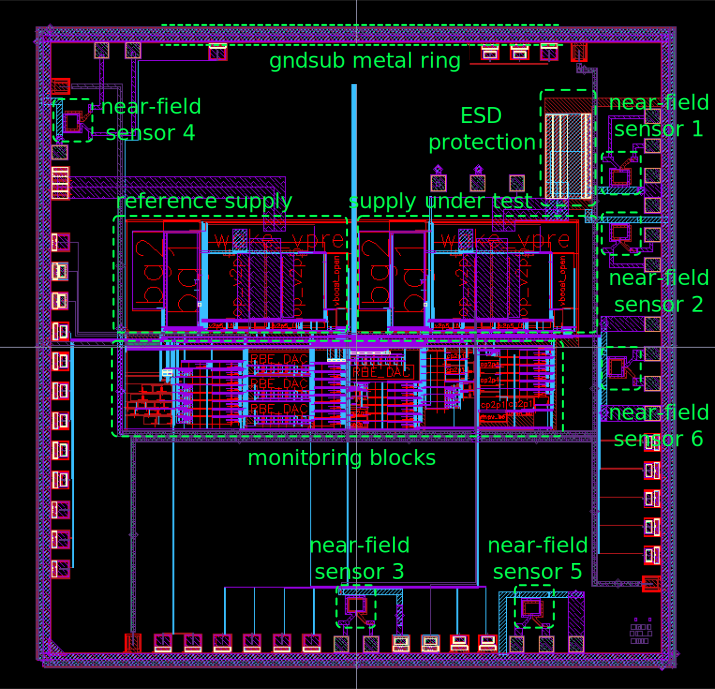
\includegraphics[width=0.7\textwidth]{src/3/figures/topcell_layout.pdf}
  \caption{Top-cell layout}
  \label{fig:top-cell-layout}
\end{figure}

% Talk about the near-field current sensors placement
In total, there are 6 near-field current sensors located on the device.
The 6\textsuperscript{th} sensor is dedicated to calibration.
The others are placed strategically on main \gls{io} susceptible to be disturbed directly or indirectly by \gls{esd}s.
Sensor \textit{1} measures the current on the supply under test power input.
During testing, this pin is be exposed to \gls{esd}s coupled on top of a DC supply voltage.
Internally, this input is protected by a large \gls{esd-protection}, able to sustain IEC 61000-4-2 \gls{esd-gun} discharges.
Sensor \textit{2} measures the current absorbed and deviated by the \gls{esd-protection} into the \textit{gndsub} metal ring (local ground reference).
Sensors \textit{3} measures the current flowing to the external stabilisation capacitor of the regulator under test.
Finally, sensors \textit{4} and \textit{5} measure the currents flowing from the \textit{gndsub} metal ring into the external ground pins, connected externally to the board ground.

% Explain why so much empty space
On the layout, a lot of silicon space was left empty.
This is due to manufacturing constraints that enforced the silicon dimensions.
After manufacturing and packaging, the chip is tested.
The entire testing process and results are documented in section \ref{sec:test-vehicle-testing}.

%TODO: Show inputs and ouputs of near-field current sensor
See Presentation "testchip" of "13 Nov 2015"
